
% NOTE: Library added, tikz

%\documentstyle[10pt,twoside]{article}
%\documentstyle[twoside]{article}
\documentclass[twoside]{article}
\setlength{\oddsidemargin}{0 in}
\setlength{\evensidemargin}{0 in}
\setlength{\topmargin}{-0.6 in}
\setlength{\textwidth}{6.7 in}
\setlength{\textheight}{8.5 in}
\setlength{\headsep}{0.75 in}
\setlength{\parindent}{0 in}
\setlength{\parskip}{0.1 in}
\usepackage{amsmath,amssymb,enumerate,algorithm,ifthen,algorithmic,epsfig, tikz}

\usetikzlibrary{automata, positioning, arrows}

% The following commands sets up the lecnum (lecture number)
% counter and make various numbering schemes work relative
% to the lecture number. Don't edit them!
%
\newcounter{lecnum}
\renewcommand{\thepage}{\thelecnum-\arabic{page}}
\renewcommand{\thesection}{\thelecnum.\arabic{section}}
\renewcommand{\theequation}{\thelecnum.\arabic{equation}}
\renewcommand{\thefigure}{\thelecnum.\arabic{figure}}
\renewcommand{\thetable}{\thelecnum.\arabic{table}}

\newtheorem{theorem}{Theorem}
\newtheorem{lemma}{Lemma}
\newtheorem{claim}{Claim}
\newtheorem{proposition}{Proposition}
\newtheorem{prob}{Problem}
\newtheorem{corollary}{Corollary}
\newtheorem{question}{Question}
\newtheorem{conjecture}{Conjecture}
\newtheorem{example}{Example}
\newtheorem{definition}{Definition}
\newtheorem{remarka}{Remark}
\newtheorem{soln}{Solution}

\def\P{\mathop{\rm P}\nolimits}
\def\NP{\mathop{\rm NP}\nolimits}
\def\DTIME{\mathop{\rm DTIME}\nolimits}
\def\BPTIME{\mathop{\rm BPTIME}\nolimits}
\def\ZPTIME{\mathop{\rm ZPTIME}\nolimits}
\def\polylog{\mathop{\rm polylog}\nolimits}

\newenvironment{remark}{\begin{remarka}\rm}{\end{remarka}}
\newenvironment{proof}{{\bf Proof.}}{\hfill\rule{2mm}{2mm}}
\newenvironment{pproof}[1]{\noindent{\textbf{Proof of #1.}}}{\hfill\rule{2mm}{2mm}}
\newcommand{\calI}{{\cal I}}
\newcommand{\calT}{{\cal T}}
\newcommand{\calP}{{\cal P}}
\newcommand{\opt}{\mbox{\sc opt}}
\newcommand{\OPT}{\mbox{\sc OPT}}
\newcommand{\QQ}{\mathbb{Q}}
\newcommand{\RR}{\mathbb{R}}
\newcommand{\ZZ}{\mathbb{Z}}
\newcommand{\DD}{\mathbb{D}}



%
% The following macro is used to generate the header.
%
\newcommand{\lecture}[5]{
   \pagestyle{myheadings}
   \thispagestyle{plain}
   \newpage
   \setcounter{lecnum}{#1}
   \setcounter{page}{1}
   \noindent
   \begin{center}
   \framebox{
	  \vbox{\vspace{2mm}
	\hbox to 6.28in { {\bf CMPUT 675: Computational Complexity Theory
						\hfill Winter 2019} }
	   \vspace{4mm}
	   \hbox to 6.28in { {\Large \hfill Lecture #1 (#2): #3 \hfill} }
	   \vspace{2mm}
	   \hbox to 6.28in { {\it Lecturer: #4 \hfill Scribe: #5} }
	  \vspace{2mm}}
   }
   \end{center}
   \markboth{Lecture #1: #3}{Lecture #1: #3}
   \vspace*{4mm}
}

%
% Convention for citations is authors' initials followed by the year.
% For example, to cite a paper by Leighton and Maggs you would type
% \cite{LM89}, and to cite a paper by Strassen you would type \cite{S69}.
% (To avoid bibliography problems, for now we redefine the \cite command.)
%
\renewcommand{\cite}[1]{[#1]}

%Use this command for a figure; it puts a figure in wherever you want it.
%usage: \fig{LABEL}{FIGURE-SIZE}{CAPTION}{FILENAME}
\newcommand{\fig}[4]{
	\begin{figure}[t]
		\begin{center}
			\includegraphics[width=#2\textwidth]{#4}
		\end{center}
		\caption{#3}
		\label{#1}
	\end{figure}
}

% Use these for theorems, lemmas, proofs, etc.

% Some useful equation alignment commands, borrowed from TeX
\makeatletter
\def\eqalign#1{\,\vcenter{\openup\jot\m@th
  \ialign{\strut\hfil$\displaystyle{##}$&$\displaystyle{{}##}$\hfil
	  \crcr#1\crcr}}\,}
\def\eqalignno#1{\displ@y \tabskip\@centering
  \halign to\displaywidth{\hfil$\displaystyle{##}$\tabskip\z@skip
	&$\displaystyle{{}##}$\hfil\tabskip\@centering
	&\llap{$##$}\tabskip\z@skip\crcr
	#1\crcr}}
\def\leqalignno#1{\displ@y \tabskip\@centering
  \halign to\displaywidth{\hfil$\displaystyle{##}$\tabskip\z@skip
	&$\displaystyle{{}##}$\hfil\tabskip\@centering
	&\kern-\displaywidth\rlap{$##$}\tabskip\displaywidth\crcr
	#1\crcr}}
\makeatother

% **** IF YOU WANT TO DEFINE ADDITIONAL MACROS FOR YOURSELF, PUT THEM HERE:

% NOW START EDITING
\begin{document}
%FILL IN THE RIGHT INFO.
%\lecture{**LECTURE-NUMBER**}{**DATE**}{**LECTURER**}{**SCRIBE**}
\lecture{0}{Eligibility}{Assignment 0}{Zachary Friggstad}{Anshil Gandhi}

% **** YOUR NOTES GO HERE:

%%%%%%%%%%%%%%%%%%%%%%%%%%%%%%%%%%%%%%%%%%
%%%%%%%%%%%%%%%%%%%%%%%%%%%%%%%%%%%%%%%%%%

\section*{Problem 1}

Give the full specification of a Turing Machine that decides the language of palindromic bit strings, including the empty string.

\soln	Denote $\epsilon$ as the blank character in a tape of a TM. Construct the following single-tape Turing Machine, $M$:

\par
$Q = \{ q_0, q_1, q_2, q_3, q_4, q_5, accept, reject \}$, where $q_0$ is the starting state of the $M$.

$\Gamma = \{ 0, 1, \epsilon \}$

Finally, the following state diagram illustrates the transition function, $\delta : Q \times \Gamma^k \rightarrow Q \times \Gamma^{k-1} \times \{ L, S, R \}^k$:




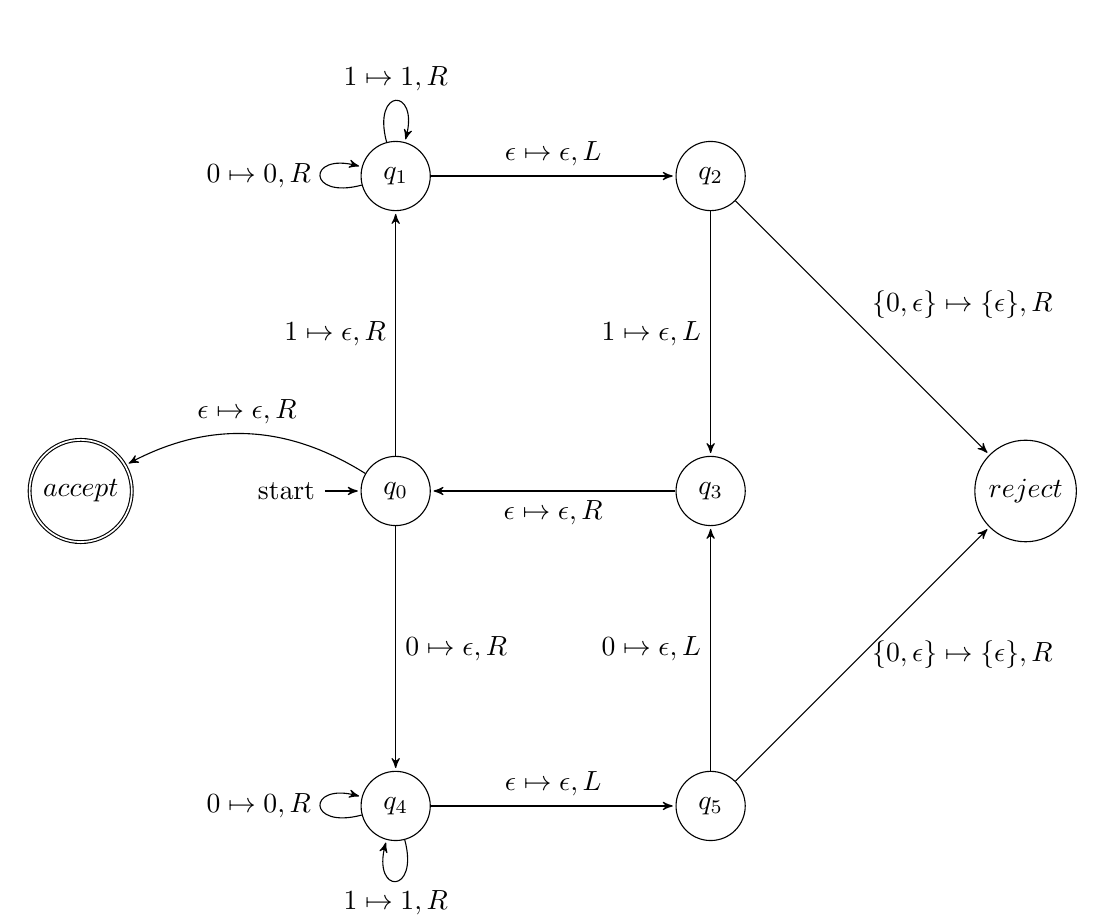
\begin{tikzpicture}[->,>=stealth',shorten >=1pt,auto,node distance=4cm,
		scale = 1,transform shape]

  \node[state,initial] (q_0) {$q_0$};
  \node[state] (q_1) [above of=q_0] {$q_1$};
  \node[state] (q_2) [right of=q_1] {$q_2$};
  \node[state] (q_3) [right of=q_0] {$q_3$};
  \node[state] (q_4) [below of=q_0] {$q_4$};
  \node[state] (q_5) [right of=q_4] {$q_5$};
  \node[state] (reject) [right of=q_3] {$reject$};
  \node[state, accepting] (accept) [left of=q_0] {$accept$};

  \path (q_0) edge              node {$1 \mapsto \epsilon, R$} (q_1)
		(q_0) edge[bend right, above]  node {$\epsilon \mapsto \epsilon, R$} (accept)
		(q_0) edge              node {$0 \mapsto \epsilon, R$} (q_4)
		(q_1) edge              node {$\epsilon \mapsto \epsilon, L$} (q_2)
		(q_1) edge[loop left]   node {$0 \mapsto 0, R$}	(q_1)
		(q_1) edge[loop above]   node {$1 \mapsto 1, R$}	(q_1)
		(q_2) edge[left]       node {$1 \mapsto \epsilon, L$} (q_3)
		(q_2) edge              node {$\{ 0, \epsilon \} \mapsto \{ \epsilon \}, R$} (reject)
		(q_3) edge              node {$\epsilon \mapsto \epsilon, R$} (q_0)
		(q_4) edge              node {$\epsilon \mapsto \epsilon, L$} (q_5)
		(q_4) edge[loop left]   node {$0 \mapsto 0, R$}	(q_4)
		(q_4) edge[loop below]   node {$1 \mapsto 1, R$}	(q_4)
		(q_5) edge              node {$0 \mapsto \epsilon, L$} (q_3)
		(q_5) edge[right]       node {$\{ 0, \epsilon \} \mapsto \{ \epsilon \}, R$} (reject);

\end{tikzpicture}






\textit{Procedure}:
\begin{enumerate}
	\item Assume the tape head of $M$ is positioned at the leftmost nonempty cell of the input/work tape. The state of
	$M$ initially is $q_0$.

	\item The transition function $\delta$ replaces the current
	value of the cell pointed by the tape head of $M$ by some
	element from $\Gamma$ and informs the tape head to either shift left, shift right or stay. Moreover, the state of $M$
	is also updated in this process. Follow the transitions provided by the state diagram above. 

	\item It is easy to see that on any input string, $M$ halts
	at either \textit{accept} or \textit{reject}. $M$ halts at
	state \textit{accept} iff the input string is a palindrome.
\end{enumerate}

%----------------------------------------------------------------
\newpage
\section*{Problem 2}
\definition	$f : \DD \rightarrow \{ 0, 1 \}^*$ is a \textit{partial} function if $f$ is well-defined on $\DD \subset \{ 0, 1 \}^*$.

\par
We say that a TM $M$ computes a partial function $f$ if:
\begin{enumerate}
\item	$\forall x \in \DD$ $M(x) = f(x)$.
\item	$\forall x \notin \DD$ M gets into an infinite loop when executed on $x$.
\end{enumerate}

If $S$ is a set of partial functions, we define $f_S : \{ 0, 1 \}^k \rightarrow \{ 0, 1 \}$ to be the boolean function that on $\alpha$ outputs $1$ iff $M_{\alpha}$ computes some partial function, $g \in S$.

\theorem(Rice's Theorem) For every nontrivial $S$ (S is a nonempty set of partial function computable by some Turing Machine and S is not maximal) $f_S$ is not computable.

% ---------------------------------------------------------------
% ---------------------------------------------------------------
\newpage
\section*{Problem 3}
\par
\theorem For any graph $G = (V, E)$ there is a mapping $f : V 
\rightarrow \{ 0, 1, 2, 3 \}$ such that $|E^*| \ge 
\frac{3}{4}|E|$, where $E^* = \{ (u, v) \in E : f(u) \ne f(v) 
\}$.
 
\par
If such an assignment exists, then $G$ is said to be almost 4-colorable.

\claim Let $G = (V, E)$ be an almost 4-colorable graph. Then $G' = (V, E \backslash \{ e_1, \cdots, e_k \})$ is also an almost 4-colorable.

\begin{proof}
Suppose $G = (V, E)$ is an almost 4-colorable graph. Then $\exists E^* \subseteq E$ such that $|E^*| \ge \frac{3}{4}|E|$. 
Now, pick an arbitrary set of edges $\{ e_1, \cdots, e_k \}$ and
remove them from $E$. Then we arrive at either of the following cases:

\par
\underline{Case 1:} $e_i, \cdots, e_j \in E^* \cap \{ e_1, \cdots, e_k \}$ $\implies$ 
	$|E^*| - j + i \ge \frac{3}{4}(|E| - j + i)$ $\implies$ $G'$ is almost 4-colorable.

\underline{Case 2:} $e_i, \cdots, e_j \in \{ e_1, \cdots, e_k \} 	\backslash E^*$. 
	$|E^*| \ge \frac{3}{4}|E| \ge \frac{3}{4}(|E| - j + i)$ and the property of almost 4-colorability still holds in $G'$.

Hence, the claim holds.

\end{proof}

\corollary 	Assume $K_n$ is almost 4-colorable, where $K_n$ is a 
	complete graph with $n$ vertices. Then any subgraph of $K_n$
	is also almost 4-colorable.

\pproof{theorem 2}

% ---------------------------------------------------------------
\end{document}
